\subsection{Arsitektur Sistem}
\label{subsection:system-architecture}

\begin{figure}[ht]
    \centering
    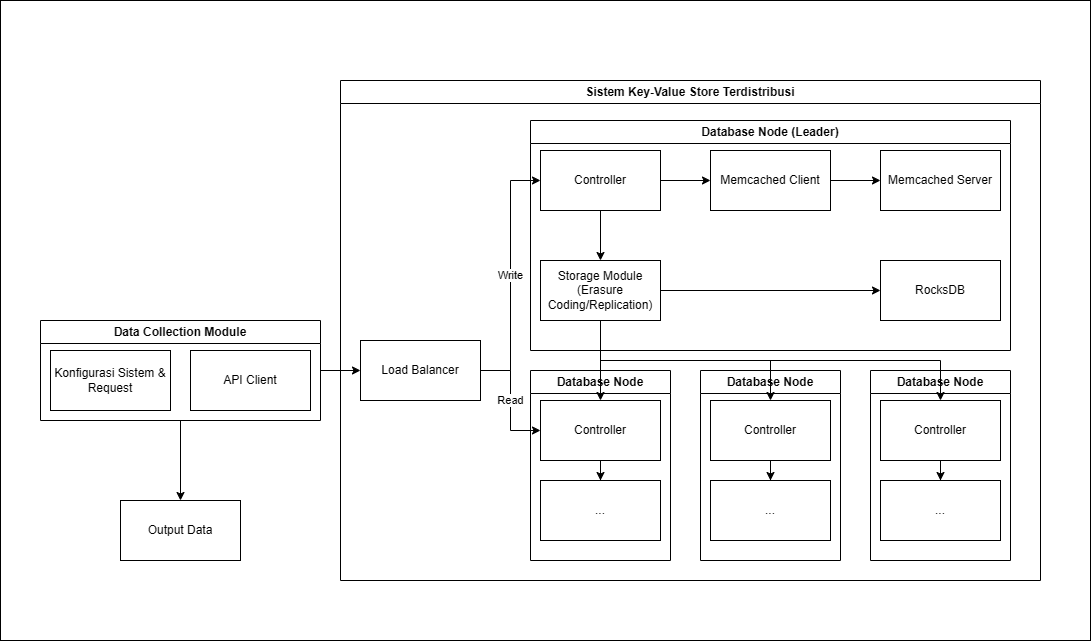
\includegraphics[width=0.95\textwidth]{resources/chapter-3/general-architecture.png}
    \caption{Gambaran Arsitektur Sistem Eksperimen}
    \label{fig:general-architecture}
\end{figure}

Arsitektur dari sistem mengasumsikan kebutuhan untuk konsistensi yang tinggi. Untuk mencapai konsistensi tersebut, operasi \textit{write} dilakukan secara \textit{synchronous} dengan distribusi replikasi dan \textit{erasure coding} dianggap selesai ketika nilai ketahanan yang diinginkan sudah tercapai.

Karena sistem bersifat terdistribusi, maka diperlukan sebuah algoritma konsensus untuk mengelola konsistensi antar \textit{node}. Algoritma konsensus yang digunakan algoritma konsensus \textit{paxos} yang disesuaikan dengan kebutuhan. Salah satu penyesuaian yang dilakukan adalah mengadopsi pola \textit{leader-follower} untuk memudahkan sinkronisasi data dan mempercepat transaksi. Dengan adanya leader, fase 1 dari algoritma \textit{paxos} dapat dihilangkan dengan membuat proposal dari leader selalu memiliki nilai paling tinggi. Detail implementasi \textit{paxos} akan dijelaskan pada modul node di bagian \ref{subsection:detail-modul}. Diagram gambaran arsitektur sistem dapat dilihat pada gambar \ref{fig:general-architecture}.

Operasi \textit{write} akan secara ekslusif disalurkan pada \textit{leader}. Kemudian untuk ketahanan, data akan didistribusikan pada \textit{follower} sesuai dengan konfigurasi modul \textit{storage}. Sementara itu, operasi \textit{read} dapat dilakukan pada \textit{database node} manapun. Pada sistem \textit{erasure coding}, jika pada \textit{node} tersebut tidak terdapat nilai data yang dicari, maka \textit{node} akan melakukan \textit{request} ke semua node lainnya untuk melakukan rekonstruksi data.
